

\newpage
\begin{figure}[t]
	\makebox[\textwidth]{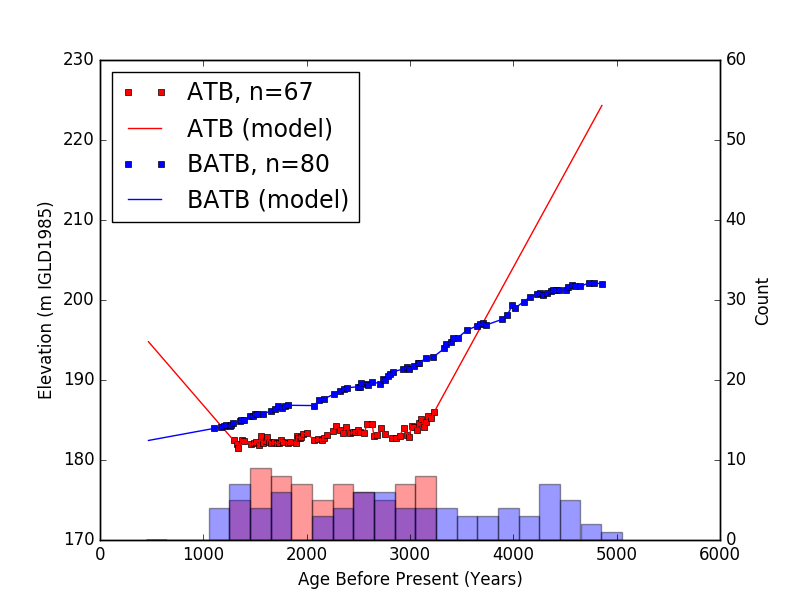
\includegraphics[width=\paperwidth]{data/ATB-BATB_DataAndModel.png}}
	\caption{Definitely not a goat.}
	\label{fig:data_ATBxBATB}
\end{figure}
\newpage

\begin{figure}[t]
	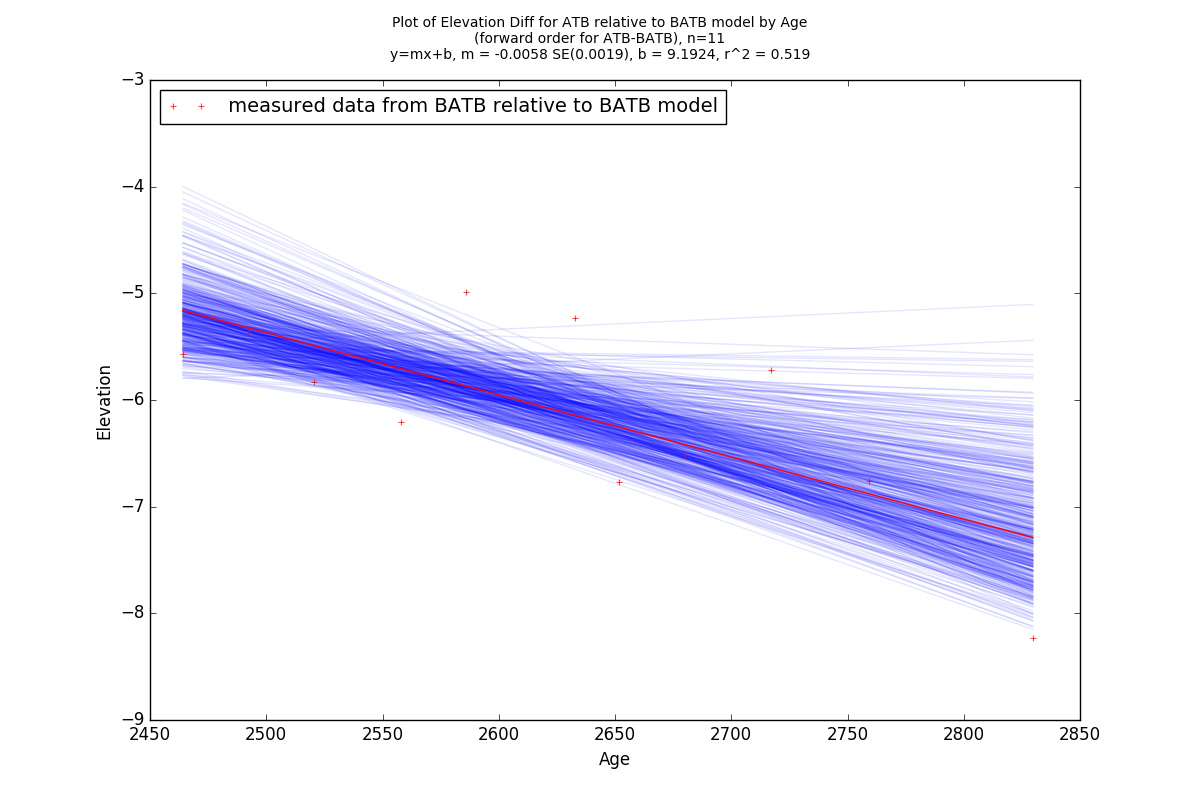
\includegraphics[width=\linewidth]{data/gias/theGIA_ATB_relative_to_BATB.png}
	\caption{Definitely not a boat.}
	\label{fig:gias_ATBxBATB}
\end{figure}
\newpage


\begin{figure}[t]
	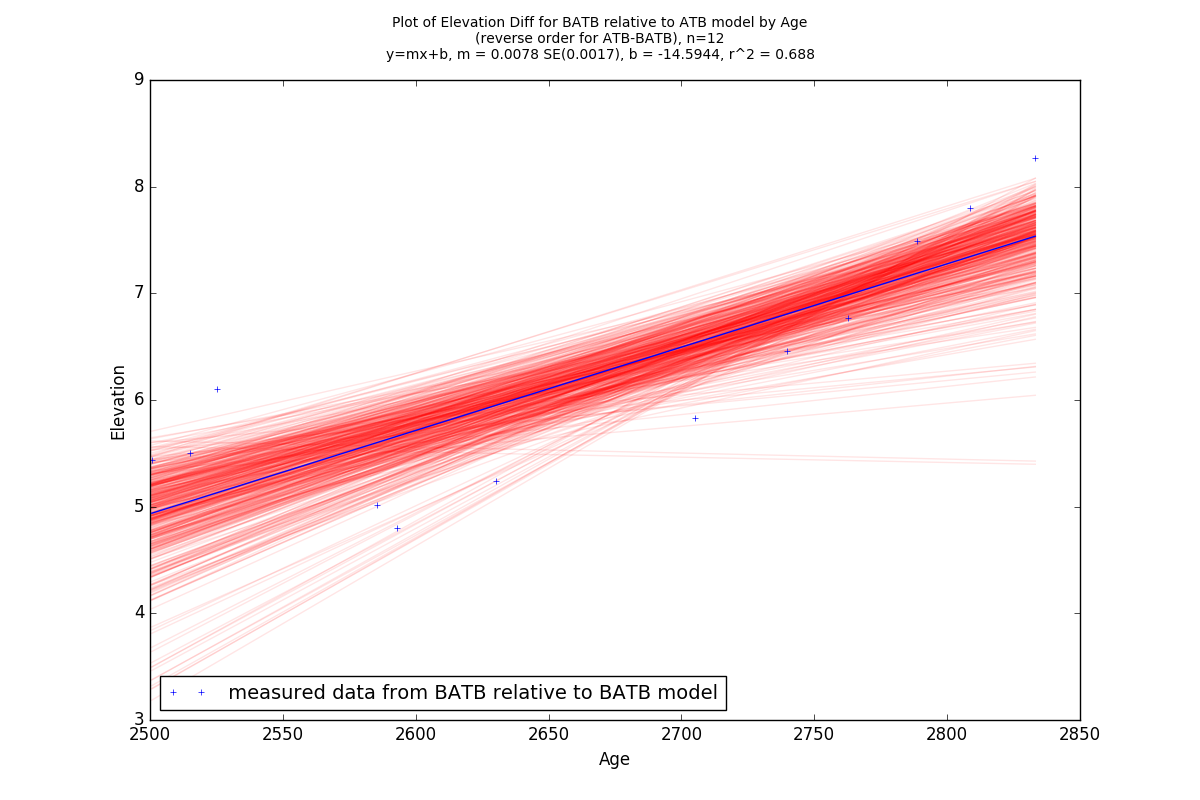
\includegraphics[width=\linewidth]{data/gias/theGIA_BATB_relative_to_ATB.png}
	\caption{Definitely not a boat.}
	\label{fig:gias_BATBxATB}
\end{figure}
\newpage
% this desperately needs to be done as a loop



\begin{figure}[h]
	\makebox[\textwidth]{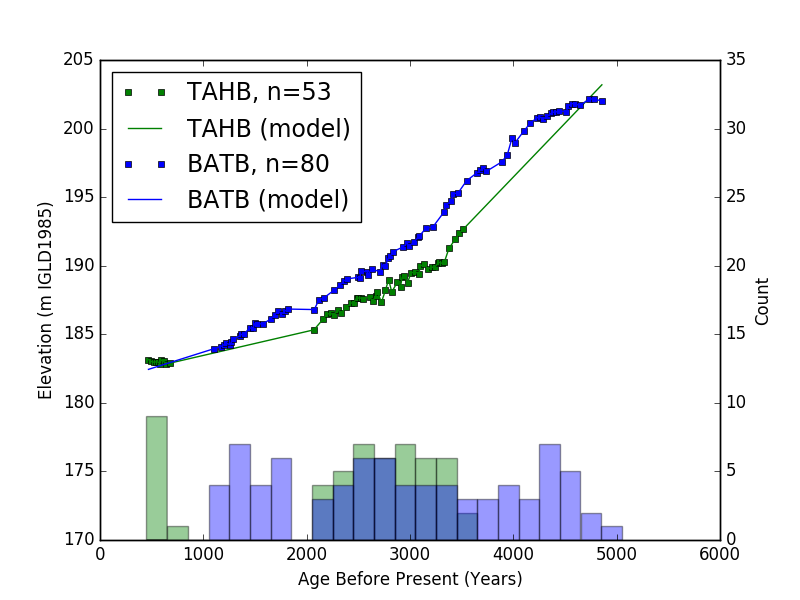
\includegraphics[width=\paperwidth]{data/TAHB-BATB_DataAndModel.png}}
	\caption{Definitely not a boat.}
	\label{fig:data_TAHBxBATB}
\end{figure}
\newpage

\begin{figure}[h]
	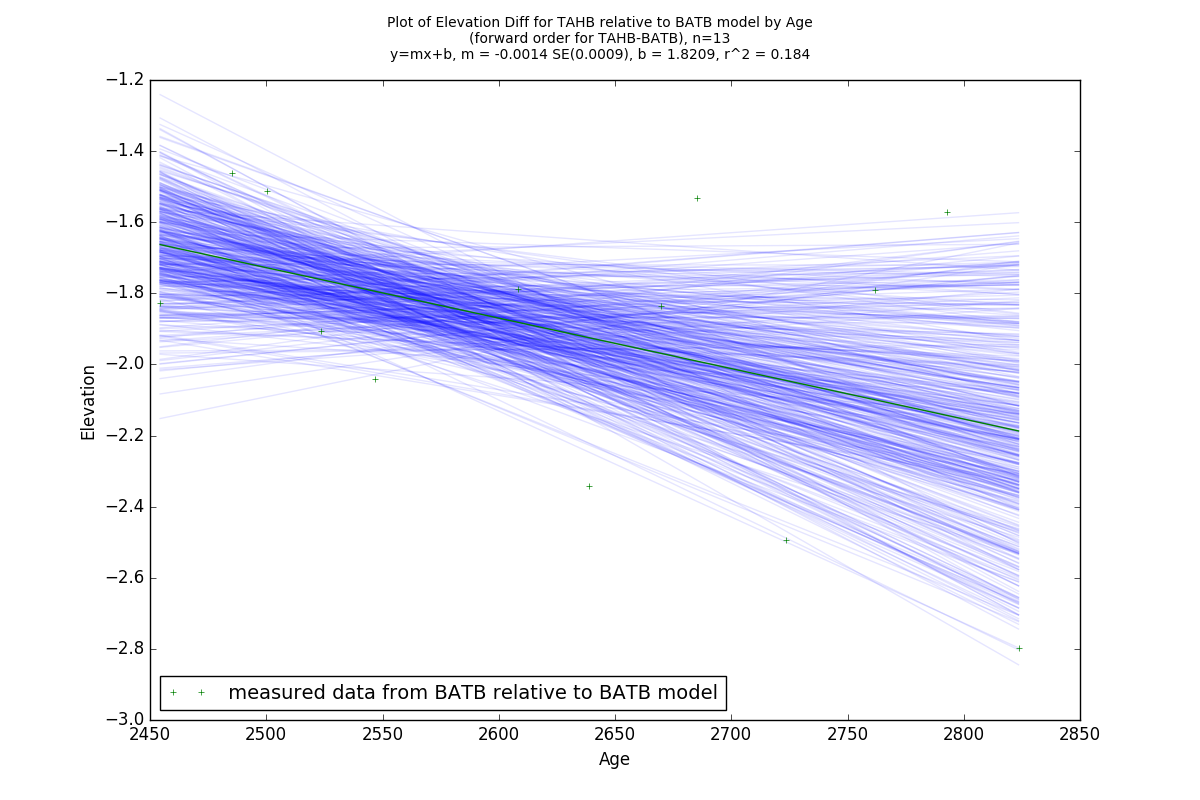
\includegraphics[width=\linewidth]{data/gias/theGIA_TAHB_relative_to_BATB.png}
	\caption{Definitely not a boat.}
	\label{fig:gias_TAHBxBATB}
\end{figure}
\newpage


\begin{figure}[h]
	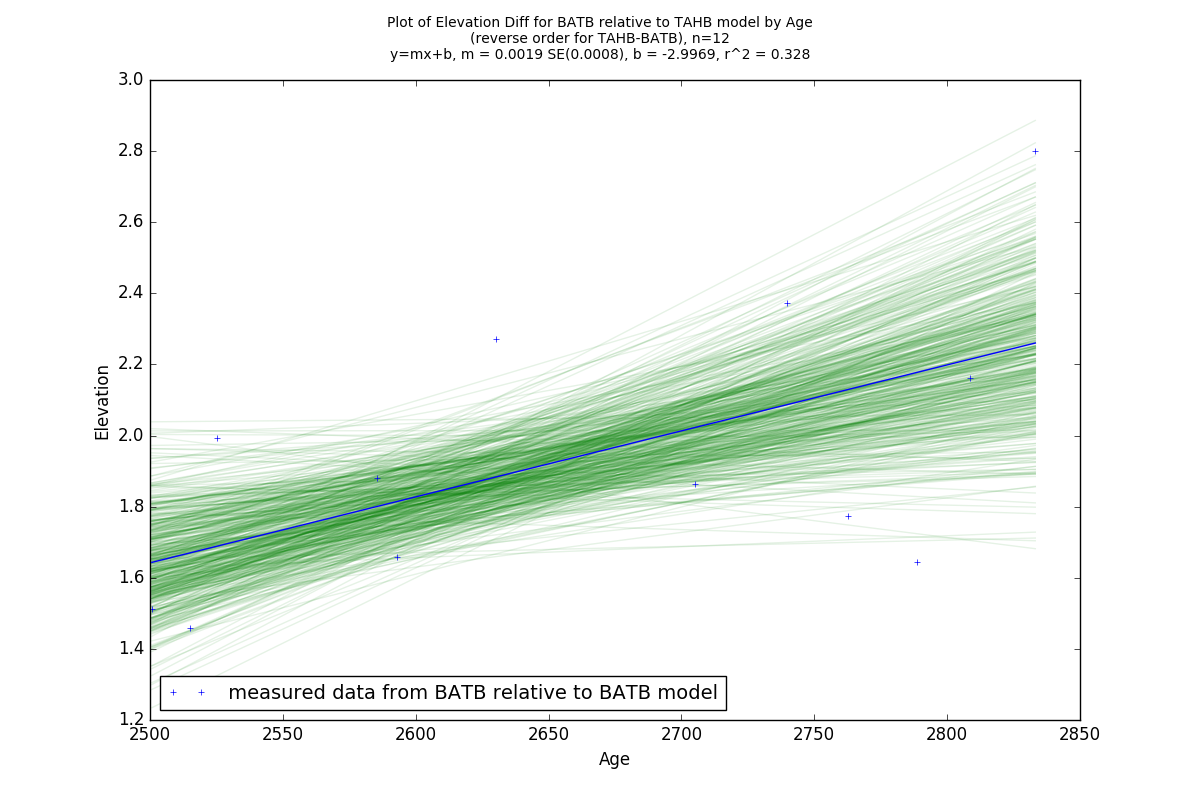
\includegraphics[width=\linewidth]{data/gias/theGIA_BATB_relative_to_TAHB.png}
	\caption{Definitely not a boat.}
	\label{fig:gias_BATBxTAHB}
\end{figure}
\newpage








\begin{figure}[h]
	\makebox[\textwidth]{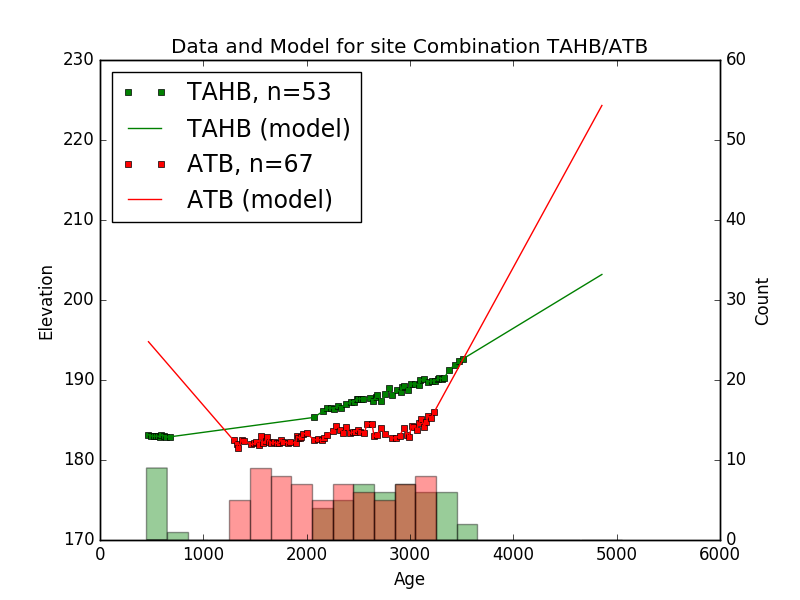
\includegraphics[width=\paperwidth]{data/TAHB-ATB_DataAndModel.png}}
	\caption{Definitely not a boat.}
	\label{fig:data_TAHBxATB}
\end{figure}
\newpage

\begin{figure}[h]
	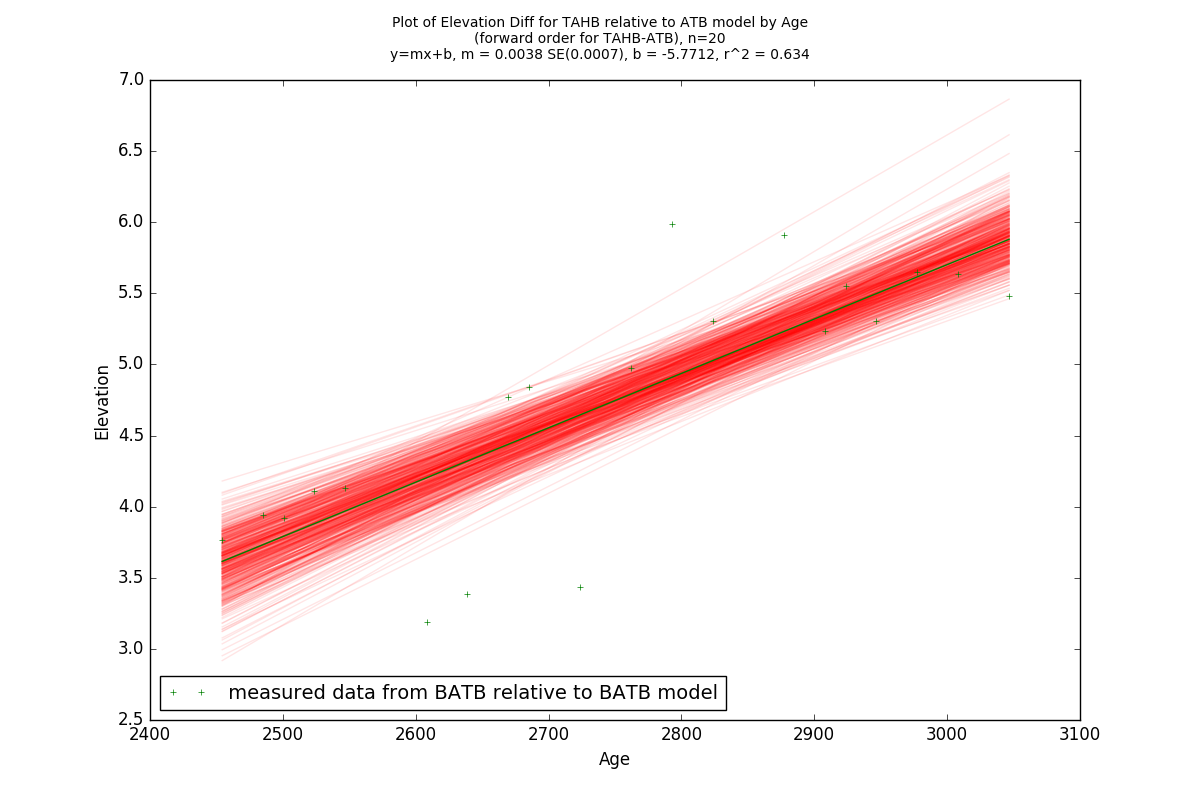
\includegraphics[width=\linewidth]{data/gias/theGIA_TAHB_relative_to_ATB.png}
	\caption{Definitely not a boat.}
	\label{fig:gias_TAHBxATB}
\end{figure}
\newpage


\begin{figure}[h]
	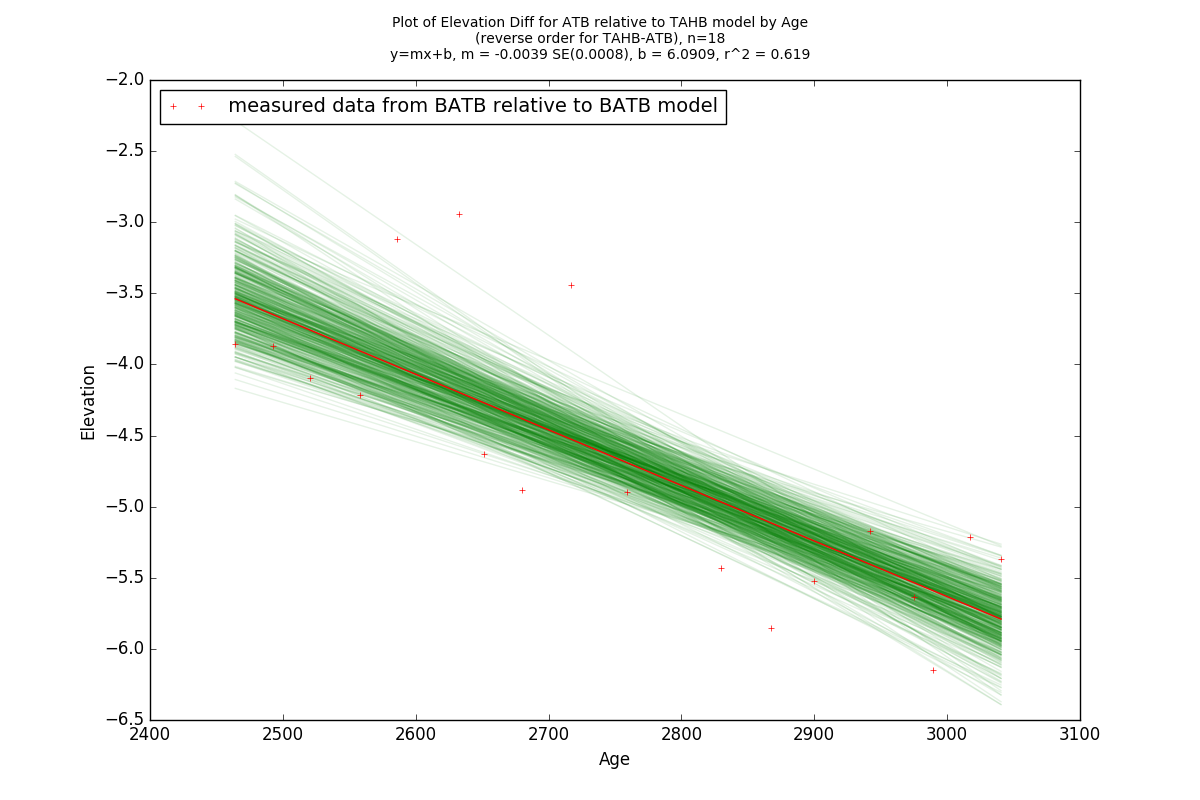
\includegraphics[width=\linewidth]{data/gias/theGIA_ATB_relative_to_TAHB.png}
	\caption{Definitely not a boat.}
	\label{fig:gias_ATBxTAHB}
\end{figure}
\newpage






\begin{figure}[h]
	\makebox[\textwidth]{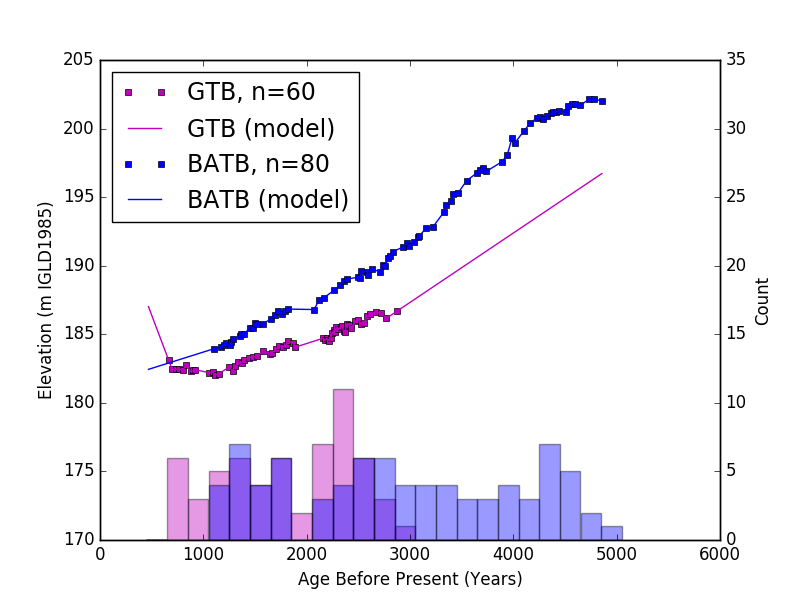
\includegraphics[width=\paperwidth]{data/GTB-BATB_DataAndModel.png}}
	\caption{Definitely not a boat.}
	\label{fig:data_GTBxBATB}
\end{figure}
\newpage

\begin{figure}[h]
	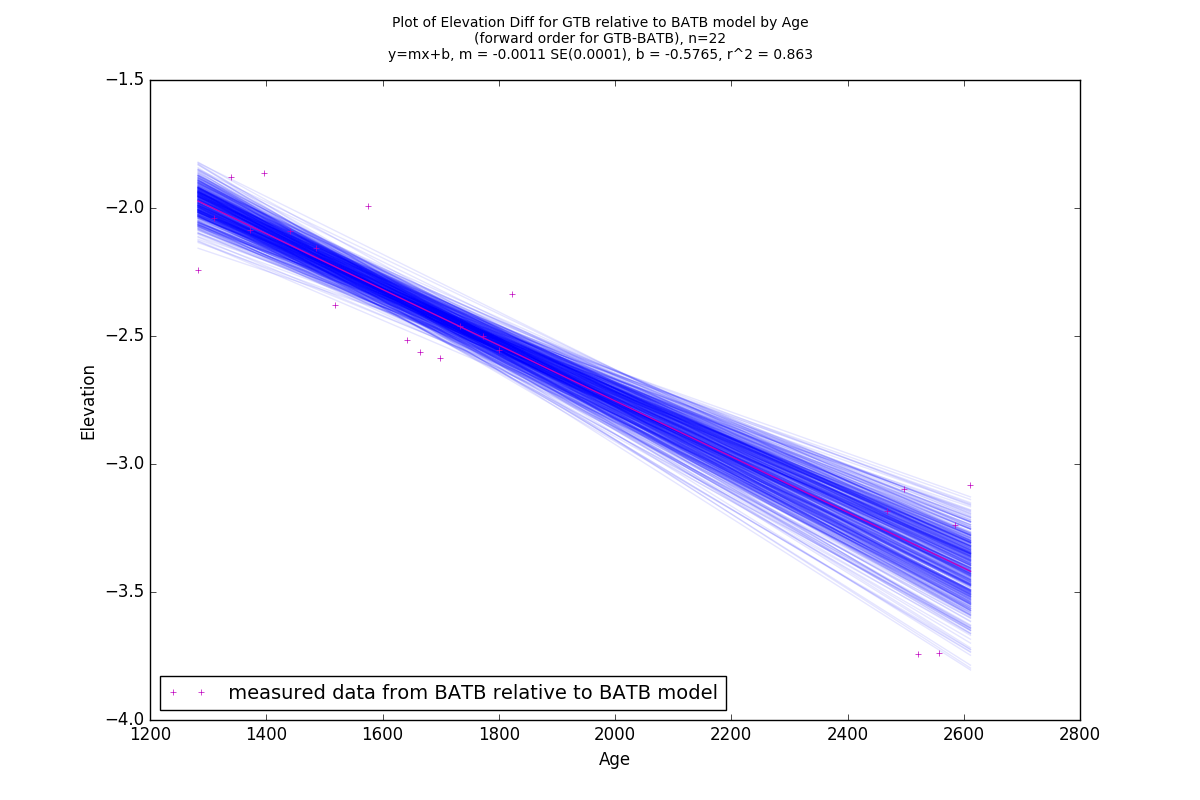
\includegraphics[width=\linewidth]{data/gias/theGIA_GTB_relative_to_BATB.png}
	\caption{Definitely not a boat.}
	\label{fig:gias_GTBxBATB}
\end{figure}
\newpage


\begin{figure}[h]
	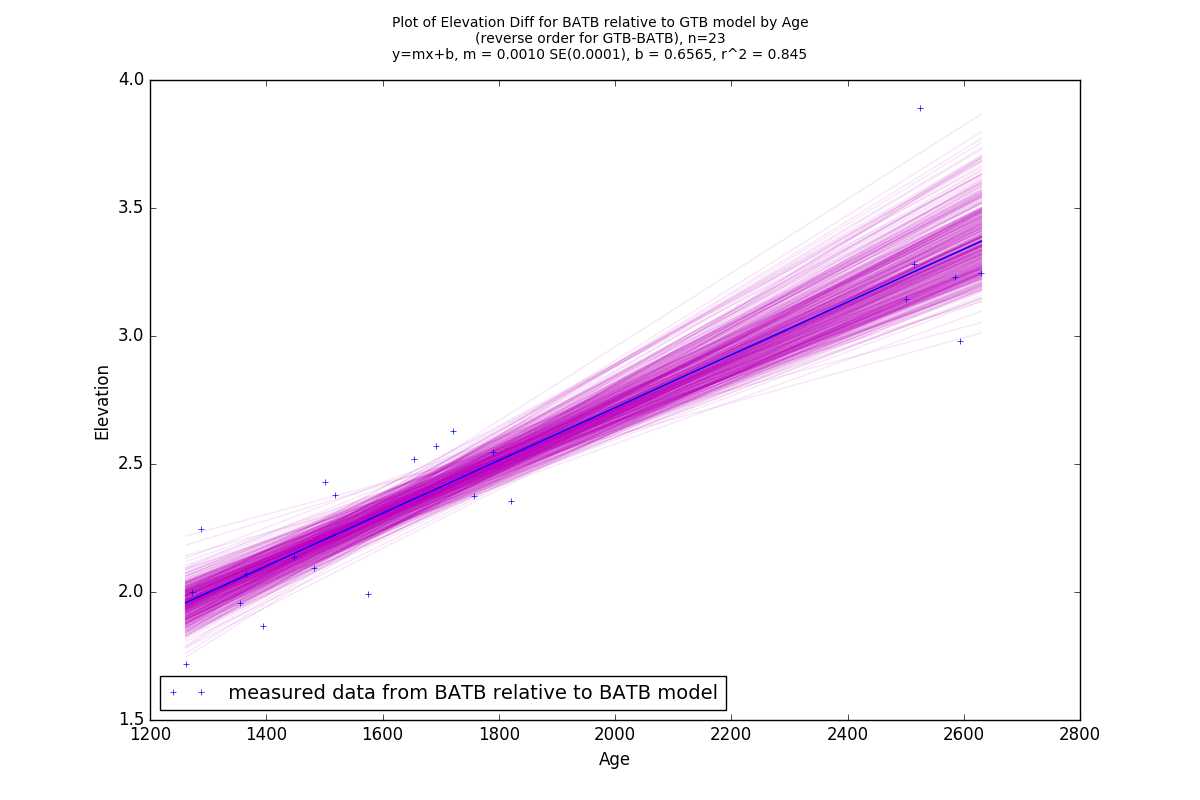
\includegraphics[width=\linewidth]{data/gias/theGIA_BATB_relative_to_GTB.png}
	\caption{Definitely not a boat.}
	\label{fig:gias_BATBxGTB}
\end{figure}
\newpage









\begin{figure}[h]
	\makebox[\textwidth]{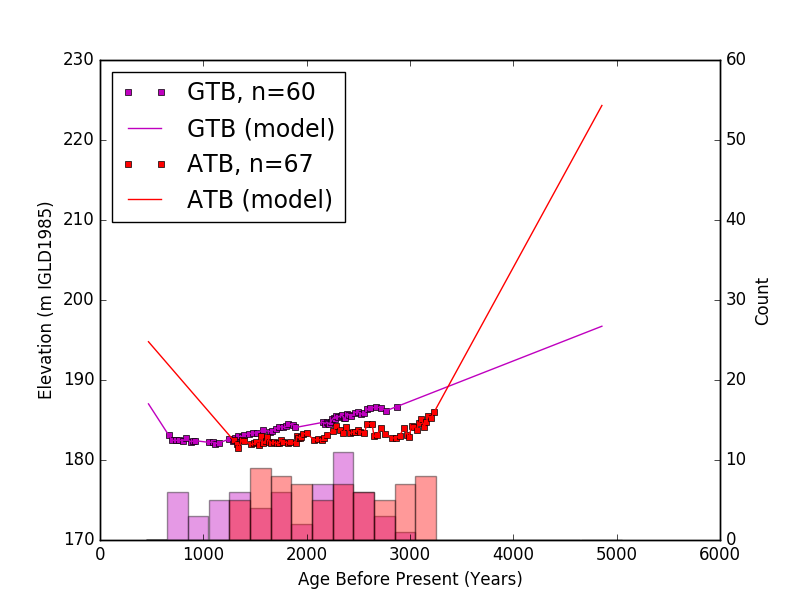
\includegraphics[width=\paperwidth]{data/GTB-ATB_DataAndModel.png}}
	\caption{Definitely not a boat.}
	\label{fig:data_GTBxATB}
\end{figure}
\newpage

\begin{figure}[h]
	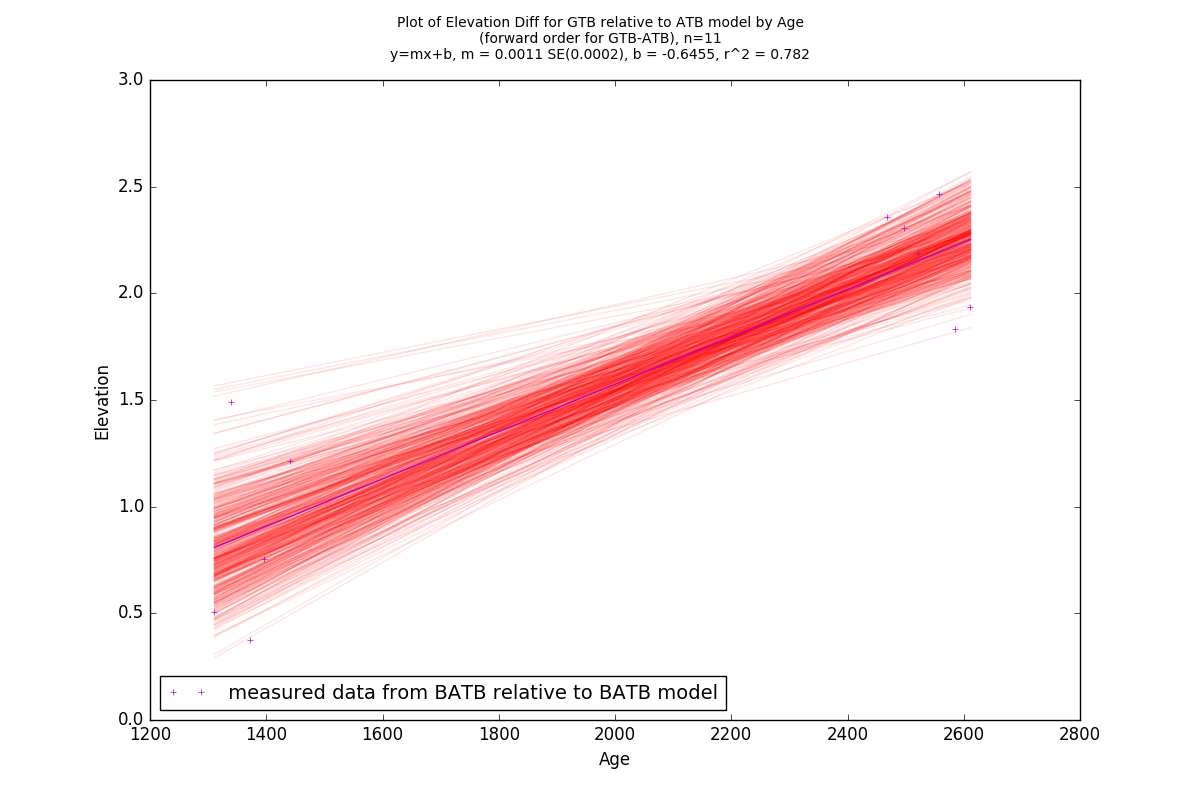
\includegraphics[width=\linewidth]{data/gias/theGIA_GTB_relative_to_ATB.png}
	\caption{Definitely not a boat.}
	\label{fig:gias_GTBxATB}
\end{figure}
\newpage


\begin{figure}[h]
	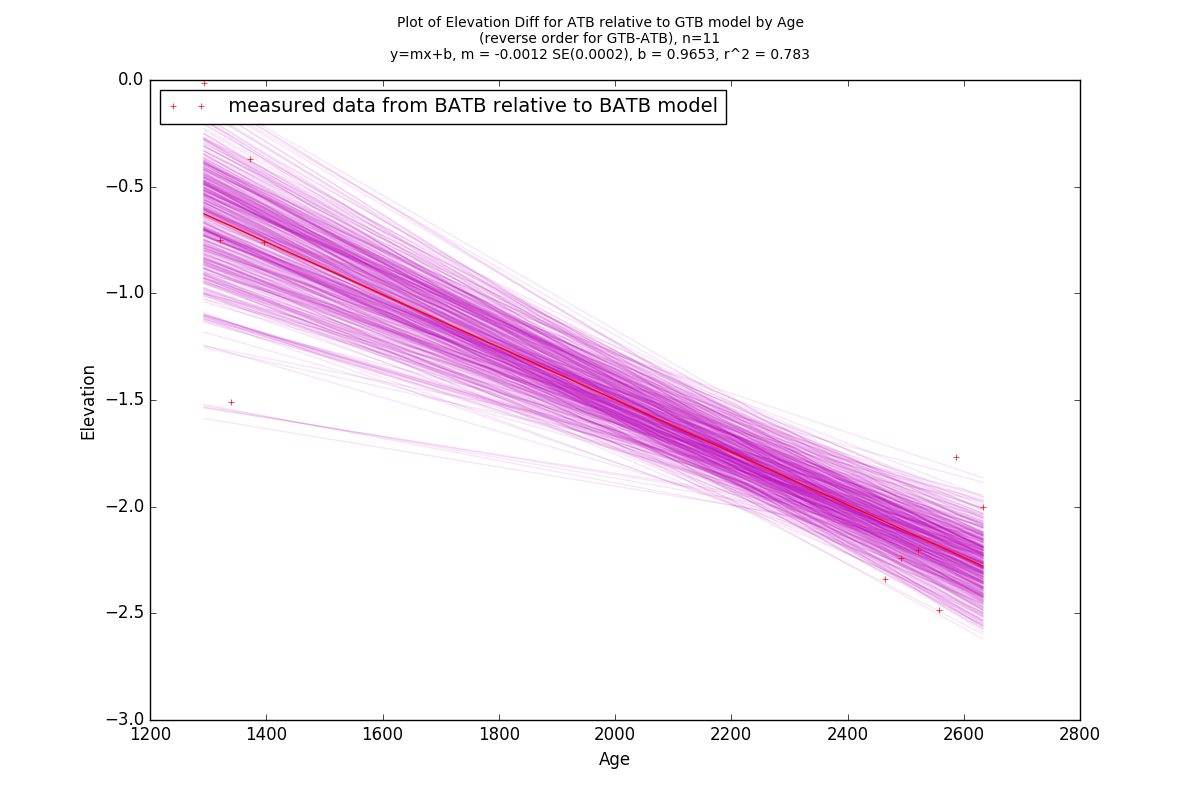
\includegraphics[width=\linewidth]{data/gias/theGIA_ATB_relative_to_GTB.png}
	\caption{Definitely not a boat.}
	\label{fig:gias_ATBxGTB}
\end{figure}
\newpage










\begin{figure}[h]
	\makebox[\textwidth]{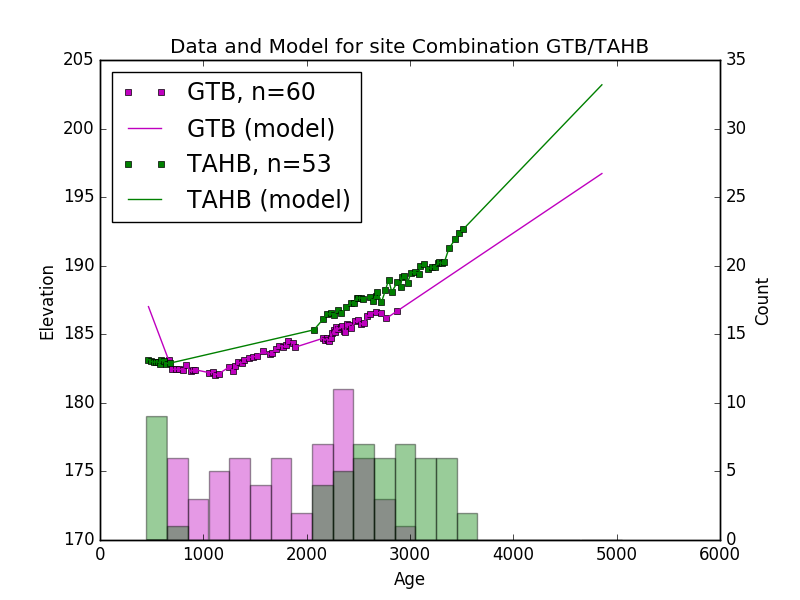
\includegraphics[width=\paperwidth]{data/GTB-TAHB_DataAndModel.png}}
	\caption{Definitely not a boat.}
	\label{fig:data_GTBxTAHB}
\end{figure}
\newpage

\begin{figure}[h]
	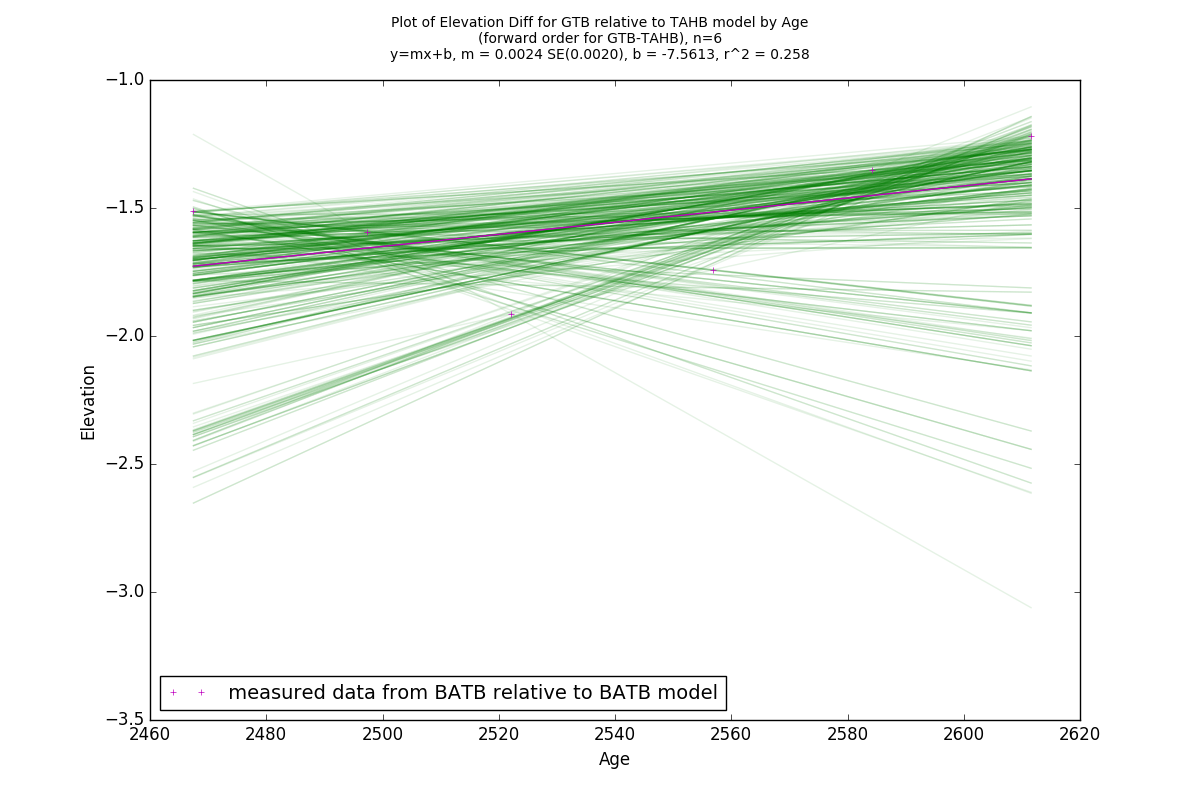
\includegraphics[width=\linewidth]{data/gias/theGIA_GTB_relative_to_TAHB.png}
	\caption{Definitely not a boat.}
	\label{fig:gias_GTBxTAHB}
\end{figure}
\newpage


\begin{figure}[h]
	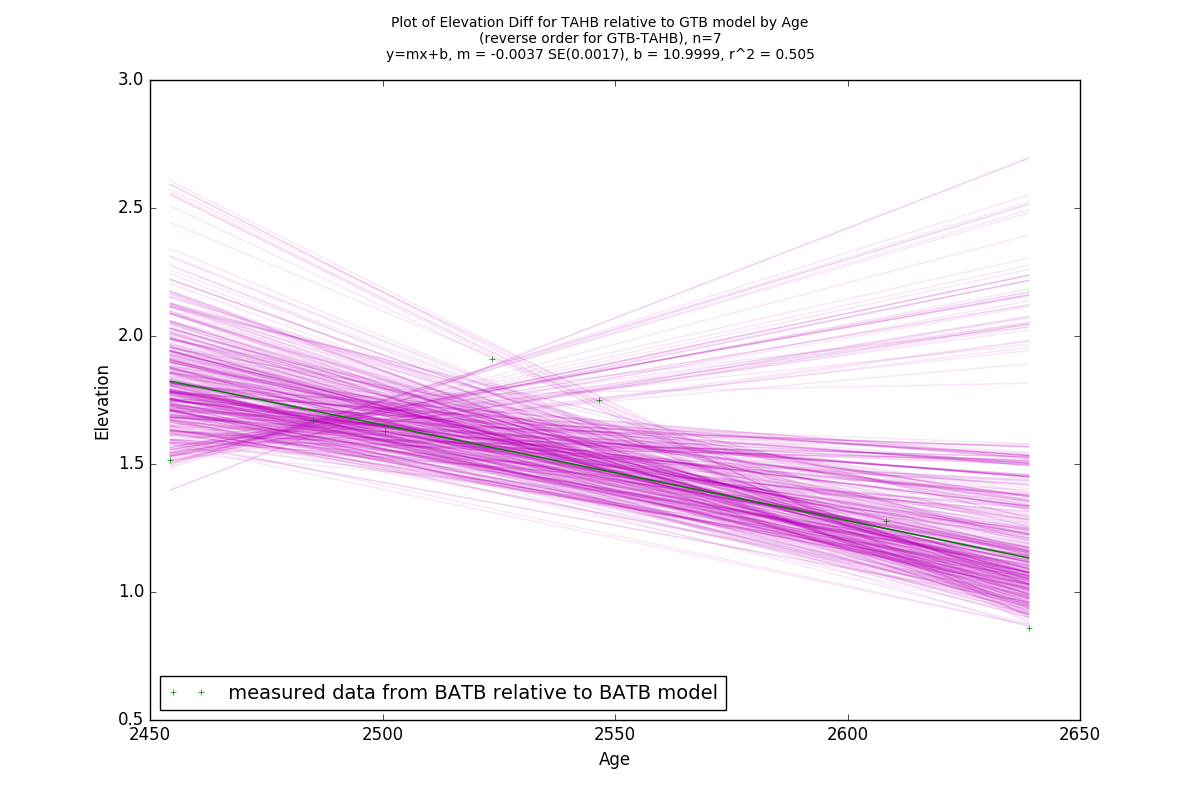
\includegraphics[width=\linewidth]{data/gias/theGIA_TAHB_relative_to_GTB.png}
	\caption{Definitely not a boat.}
	\label{fig:gias_TAHBxGTB}
\end{figure}
\newpage


\begin{figure}[h]
	\makebox[\textwidth]{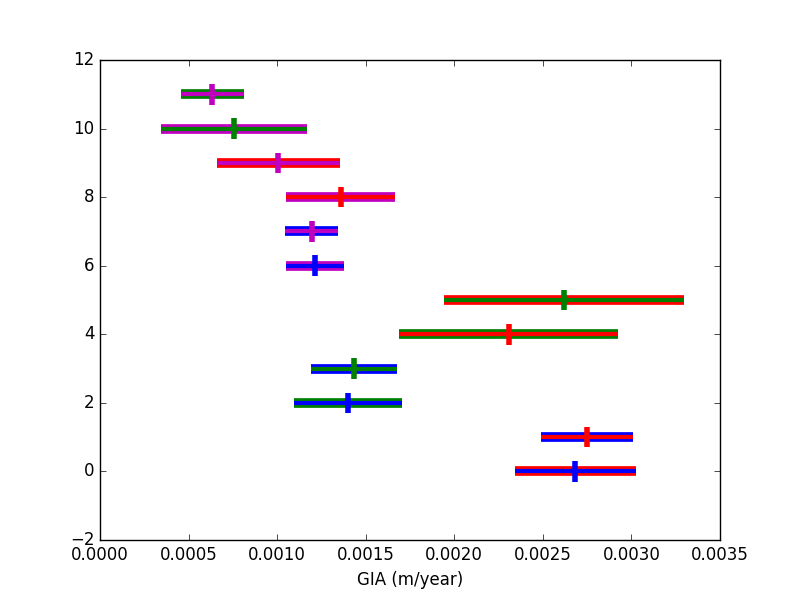
\includegraphics[width=\paperwidth]{data/intervals.png}}
	\caption{Definitely not a boat.}
	\label{fig:intervalsGIA}
\end{figure}
\newpage

